
Magnetic and electric dipoles are an effective approach for modeling the radiation of electrically small antennas. They are defined as antennas with dimensions much less than one-tenth of the wavelength ($l\ll\lambda$)\cite[p. 151]{Balanis_1997}. By calculating the respective dipole moments, the coupling between antennas and TEM cells can be numerically estimated. This section provides a brief introduction to the underlying theory of this concept.

\subsection{Electric Dipoles}

An electric dipole can be modeled as two tiny charged metal spheres or two capacitor-plates connected by a linear wire of length $d$ and diameter $a$ \cite[p. 467]{Griffiths_2024}, \cite[p. 151]{Balanis_1997}. The charges accelerate along the wire and radiate. In case of an ideal, infinitesimal dipole, the wire is very thin ($a\ll \lambda$) and very small ($d \ll \lambda$) compared to the wavelength $\lambda$ \cite[p. 151]{Balanis_1997}, \cite[p. 468]{Griffiths_2024}. For an antenna to be accurately modeled as an infinitesimal electric dipole, its length usually must be smaller than a fiftieth of the wavelength ($d < \lambda/50$) \cite[p. 156]{Balanis_1997}. They are not very practical, but serve as a basic building block for more complex geometries. The current is spatially uniform throughout the wire.

Wires that are too long to be modeled as an infinitesimal dipole, but short enough to be considered electrically small ($\lambda / 50 < l \leq \lambda/10$), are classified as short physical dipoles \cite[pp. 162-163]{Balanis_1997}. They are a more accurate and useful representation of a linear wire antenna, and investigated further. In the remainder of this thesis, the term electric dipole refers specifically to short physical electric dipoles. Furthermore, time variation according to $\mathrm{e}^{-j\omega t}$ is assumed and therefore omitted.

A current $I_0$ is fed into the short, center-fed, linear antenna shown in \autoref{fig:electric_dipole}. The current along the antenna arms $I(z)$ linearly drops to zero \cite[p. 412]{Jackson}, as visualized in \autoref{fig:electricdipolecurrent}. Mathematically, it is described by, 

\begin{equation}
    I(z)= I_0\left( 1-\frac{2|z|}{d} \right).
    \label{eqn:current_dipole}
\end{equation}


\begin{figure}[h]
    \centering
    \includegraphics[width=0.5\linewidth]{content/10_theory/img/electric_dipole_drawing.png}
    \caption{Geometrical arrangement of a linear center-fed wire antenna.}
    \label{fig:electric_dipole}
\end{figure}

Charge accumulates along the antenna's arms. It is expressed as a charge per unit length $\rho'$ due to the thin wire. It is derived by the continuity equation,

\begin{equation}
    \rho' = \pm\frac{\mathrm{d}}{\mathrm{d}z}j\frac{ I(z)}{\omega} = \pm j\frac{2  I_0}{\omega d}.
    \label{eqn:charge_distribution_dipole}
\end{equation}

$\rho'$ is uniformly distributed along each antenna arm \cite[p. 412]{Jackson}.




An important metric is the electric dipole moment $\mathbf{p}$. It is defined as the product of charge density $\rho$ along the antenna and their source point $\mathbf{x'}$ \cite[p.410]{Jackson}, and generally expressed as 

\begin{equation}
	\mathbf{p} = \iiint_V\mathbf{x'} \rho (\mathbf{x'})\,\mathrm{d}\mathbf{x'}.
	\label{eqn:elec_dipole_mom}
\end{equation}

The vector $\mathbf{x}=\mathbf{\hat{a}}_x x + \mathbf{\hat{a}}_y y + \mathbf{\hat{a}}_z z$ represents the observation point coordinates, while $\mathbf{x'}=\mathbf{\hat{a}}_x x' + \mathbf{\hat{a}}_y y' + \mathbf{\hat{a}}_z z'$ represents the source point coordinates. The vectors $\mathbf{\hat{a}}_x$, $\mathbf{\hat{a}}_y$, and $\mathbf{\hat{a}}_z$ are unit vectors along the x-, y-, and z-directions, respectively. The integration is performed over the volume $V$ of the antenna.

Knowing the charge distribution $\rho'$ enables the calculation of the electric dipole moment $\mathbf{p}$ through \autoref{eqn:elec_dipole_mom}. This results in, 

\begin{equation}
    \mathbf{p}=\int_{-\frac{d}{2}}^{\frac{d}{2}}z\rho'(z)\,\mathrm{d}z\cdot\mathbf{\hat{a}}_z = j\frac{I_0d}{2\omega}\cdot\mathbf{\hat{a}}_z.
    \label{eqn:dipole_mom_example}
\end{equation}

The electric dipole moment $\mathbf{p}$ is parallel to the antenna's arms and points in the z-direction \cite[p. 412]{Jackson}, \cite[p. 155]{Griffiths_2024}. Next, the vector potential $\mathbf{A}$ is determined. It is generally defined as  \cites[p. 152]{Balanis_1997}[p. 410]{Jackson},
 
\begin{equation}
    \mathbf{A}(\mathbf{x})=\frac{\mu}{4\pi}\frac{\mathrm{e}^{-jkr}}{r}\iiint_V \mathbf{J}(\mathbf{x'})\,\mathrm{d}\mathbf{x'}.
    \label{eqn:vector_pot}
\end{equation}


The variable $r$ is the distance from any source point to the observation point $\left| \mathbf{x}-\mathbf{x'} \right|$. The permeability is described by $\mu$ and the term $\mathrm{e}^{jkr}$ the propagation of the wave, where $k=2\pi/\lambda$ is the propagation factor, or often called wavenumber \cite[p. 704]{Balanis_1997}. $\mathbf{J}$ is the current density in the source region. The calculations of $\mathbf{A}$ simplify to \cite[p. 410]{Jackson},

\begin{equation}
    \mathbf{A} (\mathbf{x})=-j\frac{\mathrm{\mu\omega}}{4\pi}\mathbf{p}\frac{\mathrm{e}^{-jkr}}{r}
    \label{eqn:vector_pot_elec_dipole}
\end{equation}
%Should the calculation of fields even be included? I don't need them for research. But the Field equations are important for explaining the frequency behavior of the electric dipole moment. This can be done by the radiation resistance in \autoref{eqn:elec_rad_res}. In our example, the radiation power depends on the frequency squared ($\mathbf{p}$\textasciitilde

\begin{figure}[t]
	\centering
	\includegraphics[width=0.3\linewidth]{content/10_theory/img/electric_dipole_current}
	\caption{Current distribution across linear wire antenna. It has a maximum at the feedpoint, and drops to zero at points $d/2$ and $-d/2$.}
	\label{fig:electricdipolecurrent}
\end{figure}


Any other field quantities can be derived out of the vector potential $\mathbf{A}$, such as the electric field intensity $\mathbf{E}$ and magnetic field intensity $\mathbf{H}$. This is achieved in a simpler way, when first transforming the Cartesian components of $\mathbf{A}$ into spherical ones, as demonstrated by \cite[p. 153]{Balanis_1997}

\begin{equation}
	\begin{bmatrix}
		A_r  \\
		A_\theta \\
		A_\phi
	\end{bmatrix} = 	
	\begin{bmatrix}
	\sin \theta \cos \phi & \sin \theta \sin \phi & \cos \theta\\
	\cos \theta \cos \phi &  \cos \theta \sin \phi & - \sin\theta\\
	- \sin\phi  & \cos\phi  & 0
	\end{bmatrix}
		\begin{bmatrix}
		A_x  \\
		A_y \\
		A_z
	\end{bmatrix},
\end{equation}

where $\theta$ is the polar angle and $\phi$ is the azimuthal angle of the observation point $\mathbf{x}$. $\mathbf{E}$ and $\mathbf{H}$ are then expressed by \cite[p. 153]{Balanis_1997},

\begin{subequations}\label{eqn:elec_and_mag_field_dipole}
    \begin{equation}
    \mathbf{H} =\frac{1}{\mu r} \left[ \frac{\partial}{\partial r} (r A_{\theta}) - \frac{\partial A_{r}}{\partial \theta} \right]  \mathbf{\hat{\mathbf{a}}_\phi},
    \end{equation}\label{eqn:h_dipole}
    
    \begin{equation}
    \mathbf{E}=-j\omega\mathbf{A}-j\frac{1}{\omega\mu\epsilon}\nabla\left(\nabla\cdot\mathbf{A}\right).
    \end{equation}\label{eqn:e_dipole}
    
\end{subequations}

Substituting $\mathbf{A}$ into \autoref{eqn:h_dipole} and \autoref{eqn:e_dipole} reduces them to 

\begin{subequations}
	\begin{equation}
		H_r=H_\theta=0,
	\end{equation}
	\begin{equation}
		H_\phi = j\frac{k I_0 d \sin\theta}{4\pi r}\left[1 + \frac{1}{jkr}\right]\mathrm{e}^{-jkr},
	\end{equation}
\end{subequations}

and,

\begin{subequations}
	\begin{equation}
		E_r = \eta \frac{I_0 d \cos \theta}{2\pi r^2}\left[ 1 + \frac{1}{jkr} \right] \mathrm{e}^{-jkr},
	\end{equation}
	\begin{equation}
		E_\theta = j\eta \frac{kI_0 d \sin \theta }{4\pi r}\left[ 1 + \frac{1}{jkr} - \frac{1}{(kr)^2} \right] \mathrm{e}^{-jkr},
	\end{equation}
	\begin{equation}
		E_\phi = 0.
	\end{equation}
\end{subequations}

$\eta=\sqrt{\frac{\mu}{\epsilon}}$ is the wave impedance of the medium in which the waves travel.


The total radiated power of the antenna is obtained by integrating the complex Poynting vector $\mathbf{W}$ over a closed surface surrounding the antenna \cite[p. 154]{Balanis_1997}. The real part of the total radiated power provides information about energy transferred by radiation, while the imaginary part about the antenna's reactive behavior. $\mathbf{W}$ is defined by 

\begin{equation}
	\mathbf{W}=\frac{1}{2}\left(\mathbf{E}\times\mathbf{H}^*\right) .
\end{equation}

The real power transfer is derived through the time-averaged Poynting vector $\mathbf{W}_\mathrm{av}$ \cite[p. 160]{Balanis_1997}, which is calculated by

\begin{equation}
    \mathbf{W}_\mathrm{av} = \frac{1}{2} \, \Re \{ \mathbf{E} \times \mathbf{H}^* \}.
    \label{eqn:time_averaged_poynting}
\end{equation}

By integrating the time-averaged real Poynting vector $ \mathbf{W}_\mathrm{av} $ over a closed surface, the radiated power $P_{\mathrm{rad}}$ is determined. The real part of the power is independent of the integrated surface, opposed to the imaginary part. In case of an electric dipole $P_{\mathrm{rad}}$ is expressed as

\begin{equation}
    P_{\mathrm{rad}} = \frac{\mathrm{c}^2\mathrm{Z_0}\mathrm{k}^4}{12\pi}|\mathbf{p}|^2.
    \label{eqn:elec_rad_res}
\end{equation}

The radiated power increases with the frequency squared. This relation holds until the frequency is too large to consider the antenna as electrically small.

The short physical electric dipole described in this section approximate the behavior of electrically short antennas. Special care must be taken of the excitation method and shape, as it influences the behavior \cite[p. 413]{Jackson}. Additionally, any antenna investigated through this method must remain as small as possible compared to the wavelength $\lambda$, to reduce any analytical approximation errors. 

\todo[inline]{Image theory may be added for TEM cell explanations \cite[p. 184]{Balanis}}


\subsection{Magnetic Dipoles}

The magnetic dipole moment characterizes the strength of a magnetic source. A small current loop fed with a current $I_0$ can be used to model the magnetic dipole, as demonstrated in \autoref{fig:magnetic_dipole_drawing}. This relation holds as long as its overall length is smaller than a tenth of the wavelength ($l < \lambda/10$) and as long as the the wire is very thin \cite[p. 231]{Balanis_1997}. Furthermore, the radiation pattern of the magnetic dipole is equal to that of the electric dipole, with the role of the electric and magnetic fields interchanged \cite[p. 254]{Griffiths_2024}.


\begin{figure}[t]
    \centering
    \includegraphics[width=0.5\linewidth]{content//10_theory//img/magnetic_dipole_drawing.png}
    \caption{Geometrical arrangement of a current loop, fed by a current $I_0$. A magnetic current $I_\mathrm{m}$ flows along a distance $L$ perpendicular to the loop's area, which produces an equivalent magnetic dipole moment.}
    \label{fig:magnetic_dipole_drawing}
\end{figure}

The magnetic dipole moment $\mathbf{m}$ is given by \cite[p. 413]{Jackson}

\begin{equation}
    \mathbf{m}=\frac{1}{2}\iiint_V (\mathbf{x'} \times \mathbf{J})\,\mathrm{d}\mathbf{x'}.
    \label{eqn:mag_dipole_moment}
\end{equation}

Furthermore, the magnetic current $I_m$ and the electric current $I_0$ in the loop are related with \cite[p. 237]{Balanis_1997}


\begin{equation}
	I_m L = jA\omega\mu_0 I_0
	\label{eqn:magn_current_curr_loop}
\end{equation}

with $A=b^2\pi$ being the area of the current loop. Analogous to the separation distance $d$ in the electric dipole, $L$ is the length of the magnetic dipole. $I_m$ and $L$ may be used to model the magnetic dipole moment instead of the current loop. $\mathbf{E}$ and $\mathbf{H}$ are then determined with \cite[p. 237]{Balanis_1997}


\begin{subequations}
	\begin{equation}
		E_r=E_\theta=0,
	\end{equation}
	\begin{equation}
		E_\phi = -j\frac{k I_m d \sin\theta}{4\pi r}\left[1 + \frac{1}{jkr}\right]\mathrm{e}^{-jkr},
	\end{equation}
\end{subequations}

and,

\begin{subequations}
	\begin{equation}
		H_r =  \frac{I_m d \cos \theta}{2\pi r^2\eta}\left[ 1 + \frac{1}{jkr} \right] \mathrm{e}^{-jkr},
	\end{equation}
	\begin{equation}
		H_\theta = j \frac{kI_m d \sin \theta }{4\pi r\eta}\left[ 1 + \frac{1}{jkr} - \frac{1}{(kr)^2} \right] \mathrm{e}^{-jkr},
	\end{equation}
	\begin{equation}
		H_\phi = 0.
	\end{equation}
\end{subequations}

The radiated power $P_\mathrm{rad}$ of the small current loop is given by \cite[p. 238]{Balanis_1997}

\begin{equation}
	P_\mathrm{rad}=\eta\left( \frac{\pi}{12} \right) (kb)^4 \left|I_0\right|.
\end{equation}

%\autoref{fig:currentloopequcirc} shows an equivalent circuit of the small current loop. The voltage across the load is given by
%
%\begin{equation}
%	V_\mathrm{L}=V_\mathrm{oc}\frac{Z_\mathrm{L}}{Z_\mathrm{in}+Z_\mathrm{L}}.
%\end{equation}
%
%Because the source impedance is much higher than the load impedance, the voltage across the load rises while the current sinks over frequency. If the current $I_0$ is kept constant over frequency, $P_\mathrm{rad}$ would be proportional to $\omega^4$. However, due to the strongly inductive nature of the small current loops, the $I_0$ would sink quadratically over the frequency when keeping the input power equal. This leads to $P_\mathrm{rad} \propto \omega^2$, similar to the electric dipole moment. This will be shown with numerical simulations later. \todo{these two paragraphs must be explained better
%
%
%\begin{figure}[t]
%	\centering
%	\includegraphics[width=0.5\linewidth]{content/10_theory/img/current_loop_equ_circ}
%	\caption{Equivalent circuit of small current loop.}
%	\label{fig:currentloopequcirc}
%\end{figure}




\subsubsection{Crossed Dipoles}
% Read Bauernfeind's: Crossed Dipole Antennas

% When placing the magnetic dipole in the center of the upper or lower chamber of the TEM cell, and pointing in y-direction, it will generate a TEM-wave. Same goes for the electric dipole, pointing in z-direction. When combining two of these dipole moments, any excitation with the first order TEM mode is possible. This is the main idea for modeling antennas. The relation of the magnetic and electric fields is assumed to be roughly equal to the free space wave impedance. Also, magnetic dipoles create a difference in output voltage of the two ports, while electric dipoles create a increase of voltage in both ports. The power transmitted is the same. However: How are they modeled in HFSS? 

Crossed dipoles can generate a wide variety of radiation patterns. Supposed two dipoles are placed perpendicular to each other and fed 90° out of phase, an omnidirectional radiation pattern in created \cite{7293591}. If the equivalent dipoles of an EUT represents such two dipoles, any mode which can propagate in the TEM cell will do so, and therefore influence the measurement result. It is therefore not only important to know which dipoles there are representing the EUT, but also what phase and magnitude they have. Meaning that not only the dipoles aligned with the TEM mode alone influence the result. 
\todo{Write}

\todo{Dipoles next to conducting planes (balanis, collin)}

% Also, the reflections of the conducting sheets of the TEM cell might enhance the dipoles' gain, therefore artificially supporting a certain mode even more. This property is often used in antennas, where a perfect electric conductor (PEC) is placed a quarter wavelength away from the antenna, hence enhancing the gain \cite{7293591}. 

